\chapter{An Overview on Proteins}
\label{chp:proteins}

\section{Basics of Molecular Biology}
\subsection{Cells}
Life is made of cells, the fundamental working units of every living system. They are composed of water; macromolecules (proteins and polysaccharides) and other small molecules, such as lipids and amino acids. 

Cells are the smallest structural unit of an organism capable of independent functioning.Each cell follows the same common cycle of birth, replication, protein synthesis and death. 

\subsection{DNA}
The nucleus of the cell contains the DNA, which contains the genetic information of the individual, the DNA is highly folded to save up as much space in the nucleus.

The genome is an organism's complete set of DNA, the human genome contains about 3 billion DNA base pairs and 24 distinct chromosomes.  

\begin{figure}[h]
	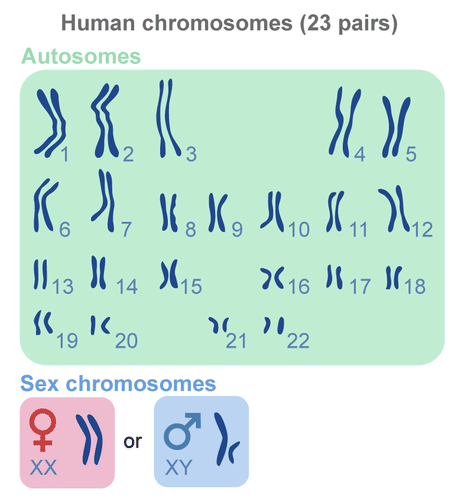
\includegraphics[scale=0.8]{res/proteins_overview/chromosomes.png}
	\caption{Chromosomes set in human genome, from \cite{chromosomes}}
	\label{fig:chromosomes}
\end{figure}

In figure \ref{fig:chromosomes} we can see the set of 24 chromosomes in the human genome. A cell normally contains 23 chromosomes, the 22 common ones, the autosomes, plus one of the sex chromosomes, "XX" in females and "XY" in males.

Chromosomes are contains pieces of DNA, among them we have genes: the basic functional units of heredity.

Genes are specific sequences of DNA that encode instructions on how to make proteins, they determine the principal hereditary characteristics in the human being, such as height, muscular mass and appetite.

Mutations of one or more genes can cause alterations as harmless as a different eye color or as serious as a disease. These mutations can also provide beneficial effects, such as immunity or protection for some diseases, for example a specific gene mutation is known for its protection against malaria.


The DNA can be used to synthesize proteins, particular molecules that participate in most of the essential processes of the human body:
\begin{itemize}
	\item building and repairing body structures;
	\item digesting nutrients;
	\item hormones: some hormones are proteins or protein-derived. Hormones are chemical messengers that flow through blood to coordinate different body's functions;
	\item executing various metabolic functions, or assisting the execution.
\end{itemize}

\subsection{Central Dogma of Biology}

The Central Dogma of Biology describes the transfer of genetic information from DNA to RNA to proteins. The key steps involved are :
\begin{itemize}
    \item \textbf{Replication}: Duplication of DNA molecules, used during cell division;
    \item \textbf{Transcription}: Synthesis of an RNA molecule, using DNA as template;
    \item \textbf{Translation}: Synthesis of a protein, using the information encoded in RNA molecules.
\end{itemize}
Now I will describe the Transcription step, that produces RNA molecules and the Translation step, that synthesize proteins.


\subsubsection{Transcription}
Transcription is the process of copying a segment of DNA into RNA.

\begin{figure}[h!]
	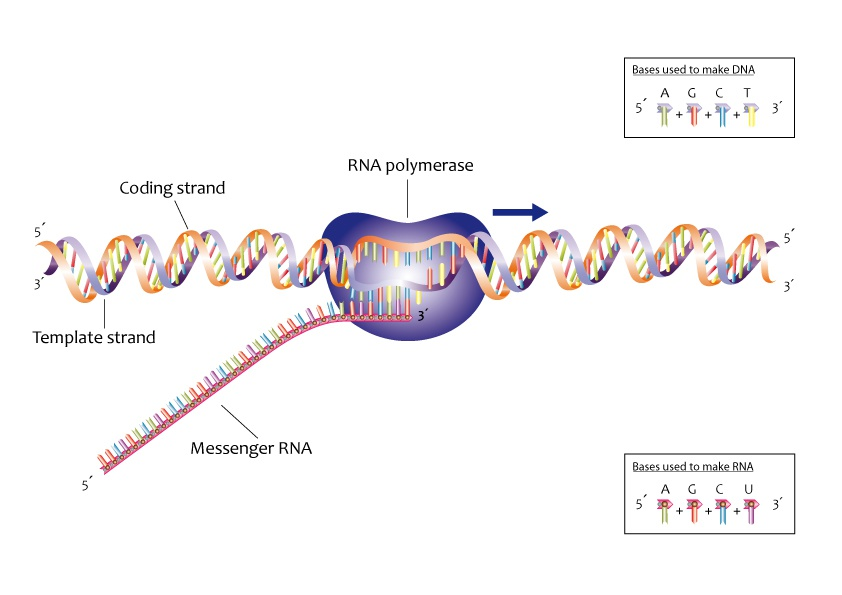
\includegraphics[scale=.53]{res/proteins_overview/rna_polymerase.jpeg}
	\centering
	\caption{Transcription: RNA Synthesization, from \cite{transcription}}
	\label{fig:transcription}
\end{figure}

An enzyme called RNA polymerase produces an RNA strand, by passing through a DNA strand. 

The resulting RNA is the copy of the coding strand of the "input" DNA , while the strand used as template to create this copy is called template strand.

In figure \ref{fig:transcription} we can see how RNA polymerase creates the RNA. We can note that the RNA molecule is called messenger RNA, also known as \textbf{mRNA}.

There are other two types of RNA, tRNA and rRNA. Let's see the differences:
\begin{itemize}
	\item \textbf{mRNA}: messenger RNA, contains the genetic information from the DNA. mRNA specifies ;
	\item \textbf{tRNA}: transfer RNA, transfer the correct amino acid to the ribosome. It acts as a bridge between the mRNA and the ribosome;
	\item \textbf{rRNA}: ribosomal RNA, combined with ribosomal proteins creates the ribosome.
\end{itemize}

\subsubsection{Translation}

Translation is the cellular process that synthesizes proteins based on the genetic instructions encoded in messenger RNA.

\begin{figure}[h!]
	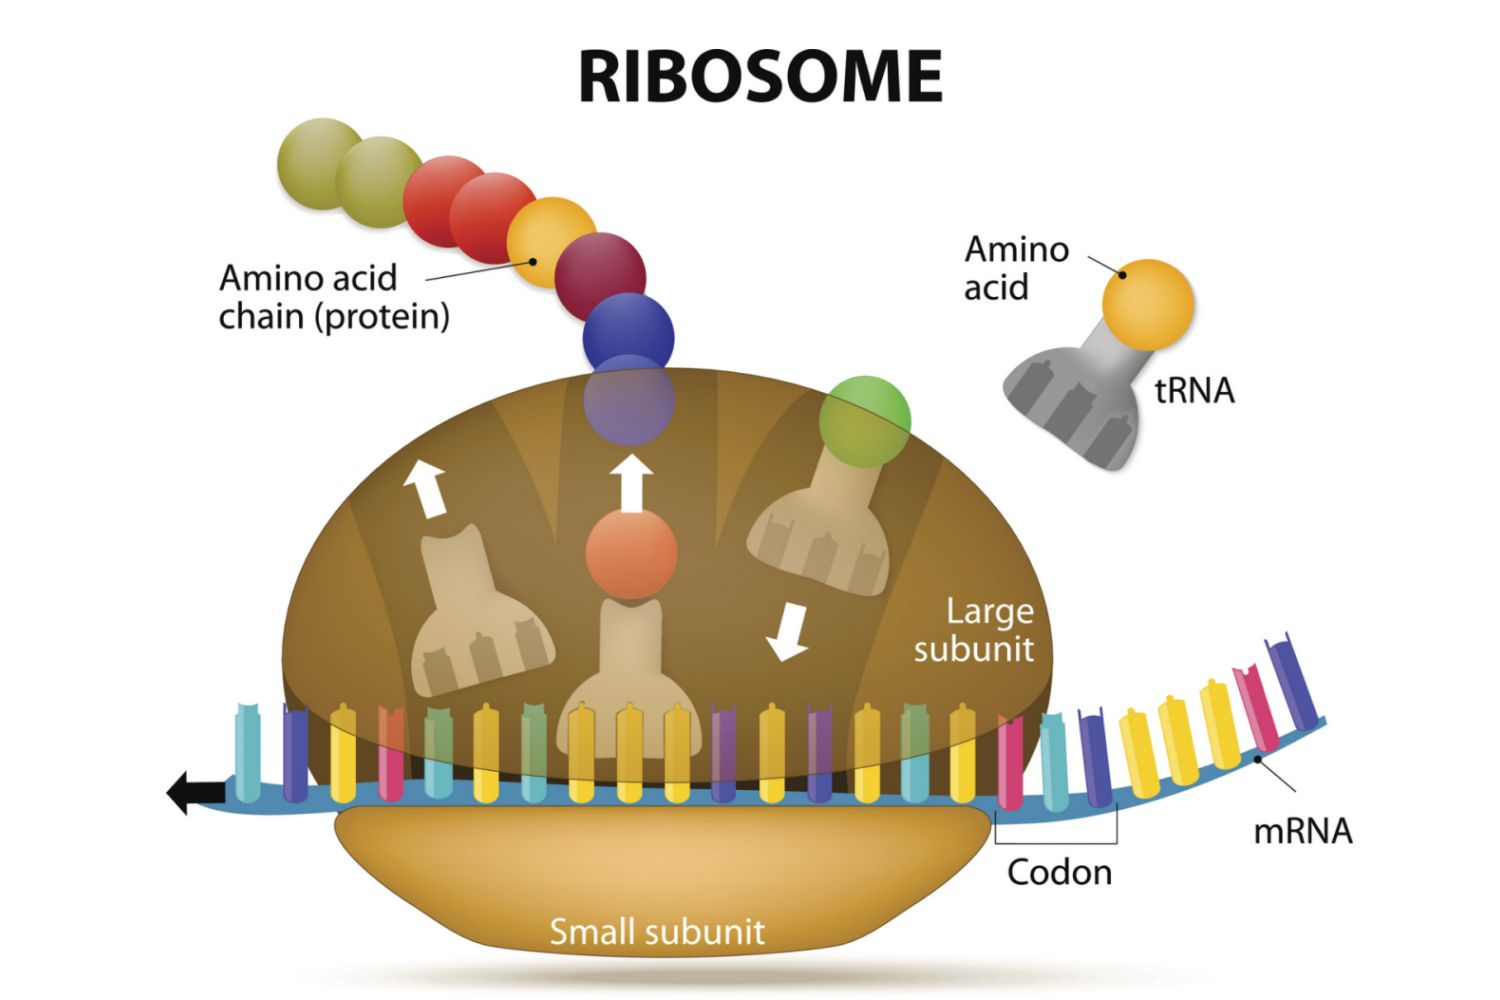
\includegraphics[scale=.3]{res/proteins_overview/ribosome.png}
	\centering
	\caption{Translation: Protein Synthesization, from \cite{translation}}
	\label{fig:protein-synth}
\end{figure}

In figure \ref{fig:protein-synth} we can how the ribosome synthesizes the protein chain.

The synthesization happens inside a ribosome, which reads the triplet of nucleotides of the mRNA (\textbf{codon}) and brings the correct tRNA, which has a triplet of nucleotides (\textbf{anticodon}) that matches the codon.

Then the tRNA transfers its amino acid to the growing protein chain of the ribosome.

In figure \ref{fig:protein-synth} we can see how the ribosome, along with tRNAs, identifies the correct amino acid and transfers it into the growing protein, through a chemical bond.

\begin{figure}[h!]
	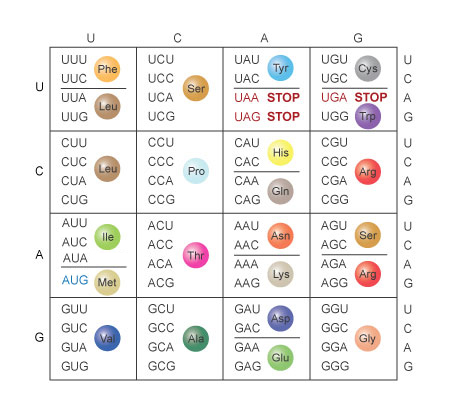
\includegraphics[scale=1.3]{res/proteins_overview/genetic_code.png}
	\centering
	\caption{Genetic code, from \cite{geneticcode}}
	\label{fig:genetic-code}
\end{figure}

In the figure \ref{fig:genetic-code} above, we can observe the Genetic Code: the set of triplets of nucleotides, codons and the corresponding amino acid.

We can observe 4 particular combinations of nucleotides that correspond to signal of start and stop the protein synthesization:
\begin{itemize}
	\item The codon \textbf{AUG} identifies the \textbf{START} signal for the protein translation;
	\item The codons \textbf{UAA, UAG, UGA} identify the \textbf{STOP} signal, which ends the translation process producing the final protein.
\end{itemize}
\vspace{5em}
\subsection{Proteins}
Proteins are large, complex molecules made up of amino acids, smaller subunits also referred to as residues. The residues are the building blocks of a macromolecule, so in this case the residues are the incorporated amino acids.
Proteins are linear chains of different combinations of 20 different amino acids. 

\subsubsection{Protein Functions}
\begin{itemize}
	\item Cellular structure;
	\item Present in body's major components, such as skin and hairs;
	\item Hormones, some of them are proteins, they communicate with other cells;
	\item Enzymes are proteins, they regulate gene activity.
\end{itemize}

The protein function depends both on the amino acids' sequence order and types and on the three-dimensional structure the protein folds into.

\subsubsection{Protein Folding}
Proteins tend to fold into lowest energy three-dimensional conformation. They already begin to fold already when the amino acid chain is being formed during translation.

Different amino acids have different chemical properties and by interacting with each other the protein starts to fold adopting its functional structure.

The structure of the protein determines the protein function. Through folding some amino acids are more exposed, this determines which substrates the protein can react to.

Substrates are molecules or compounds that participate in a chemical reaction, they are starting materials or reactants which are acted upon by enzymes or catalysts.
\vspace{6em}
\pagebreak

\begin{figure}[h!]
	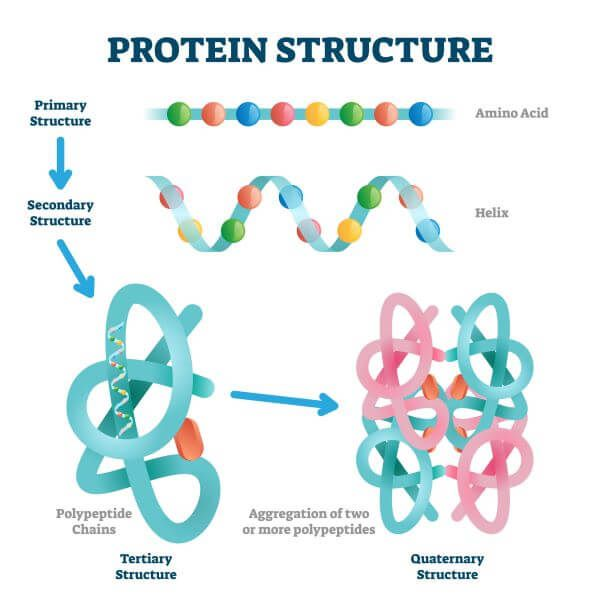
\includegraphics[scale=0.75]{res/proteins_overview/protein_structure.png}
	\centering
	\caption{Structure of proteins, from \cite{structureproteins}}
	\label{fig:protein-structure}
\end{figure}

From figure \ref{fig:protein-structure} we can see the four types of structures in a protein:

\begin{itemize}
	\item \textbf{Primary structure}: the sequence of amino acids;
	\item \textbf{Secondary structure}: local structural patterns formed by residues;
	\item \textbf{Tertiary structure}: the global structure of the peptide chain;
	\item \textbf{Quaternary structure}: aggregation between the various peptide chains in the protein. 
\end{itemize}

\vspace{2em}

The main two types of secondary structures are :

\begin{itemize}
	\item \textbf{Alpha-helix}: proteins bury most of their hydrophobic residues in the interior core, forming a spiral structure resembling an helical spring;
	\item \textbf{Beta-sheets}: segments of the protein are stretched out and aligned in a sheet-like arrangement.
\end{itemize}
\vspace{6em}
\pagebreak
\subsubsection{Amino Acids}
Amino acids are monomers\footnote{A monomer in molecular biology is a molecule that can bond with other monomers to create a macromolecule. } of proteins, each amino acid has a specific chemical behavior.

All amino acids in the human genetic code have a carboxyl group (-COOH) and an amino group (-NHH) bound to the central carbon atom. Amino acids differ for the side chain, while the carboxyl group and the amino group are the same for each one of the 20 amino acid. Side chains differ in these 3 features :
\begin{itemize}
	\item three-dimensional structure;
	\item electric charge;
	\item hydrophobicity.
\end{itemize}

Amino acids are mainly classified by hydrophobicity :
\begin{itemize}
	\item hydrophobic amino acids repel water, they are also called non-polar amino acids. 
	\item hydrophilic amino acids are attracted to water, they are also called polar amino acids.
\end{itemize}
\pagebreak
Other classifications take into account the structure, functionality or electrical charge of the amino acid (uncharde, positively charged or negatively charged). Some other classifications are based on the particularity of the side chains, such as Sulfur-Containing.

\begin{table}[h!]
\begin{tabular}{ c|c|c|c }
	 & & & \\
	\textbf{Full Name} & \textbf{Abbreviation} & \textbf{Abbreviation} & \textbf{Polarity} \\
	 & \textbf{(3 Letters)} & \textbf{(1 Letter)} & \\
	\hline
 Glycine & Gly & G & \\  
 Alanine & Ala & A & \\ 
 Valine & Val & V & \\
 Leucine & Leu & L & \\
 Isoleucine & Ile & I & Non-Polar \\
 Methionine & Met & M & \\
 Phenylalanine & Phe & F & \\
 Tryptophan & Trp & W & \\
 Proline & Pro & P & \\
 	\hline
 Serine & Ser & S & \\
 Threonine & Thr & T & \\
 Cysteine & Cys & C & \\
 Tyrosine & Tyr & Y & \\
 Asparagine & Asn & N & \\
 Glutamine & Gln & Q & Polar \\
 Aspartic Acid & Asp & D & \\
 Glutamic Acid & Glu & E & \\
 Lysine & Lys & K & \\
 Arginine & Arg & R & \\
 Histidine & His & H & \\

\end{tabular}
\caption{List of Amino Acids}
\label{table:amino-acids}
\end{table}

\vspace{2em}

In the table \ref{table:amino-acids}, we can see the list of the 20 amino acids in the Genetic Code with :
\begin{itemize}
	\item Polarity;
	\item Three letters abbreviation;
	\item One letter abbreviation.
\end{itemize}

To check which triplet of nucleotides corresponds to each amino acid in the Genetic Code, we can go back to figure \ref{fig:genetic-code}.

\vspace{10em}

\subsection{Tandem Repeat Proteins}
Tandem repeat proteins are the product of minimal folds from the repetition of simpler units. Their buried residues are more conserved, with a large surface and a high sequence variability.

\begin{figure}[h!]
	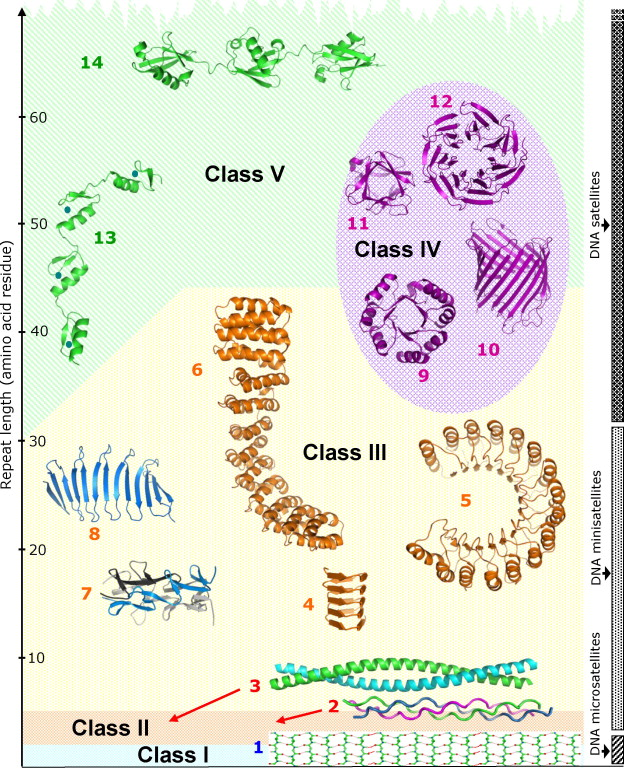
\includegraphics[scale=0.6]{res/proteins_overview/tandem.jpg}
	\centering
	\caption{Tandem Repeat Proteins, from \cite{tandem}}
	\label{fig:tandem}
\end{figure}

From the figure \ref{fig:tandem} we can see what tandem repeat proteins look like. We can also observe how they are divided into classes; tandem repeat proteins are classified according to periodicity in 5 classes:
\begin{itemize}
	\item Class I: Aggregates;
	\item Class II: Collagen and Coiled-coils;
	\item Class III: Solenoids;
	\item Class IV: Toroids;
	\item Class V: Beads on a string.
\end{itemize}

\subsection{Intrinsically Disordered Proteins}
A polypeptide chain can be classified as different types of proteins, such as:
\begin{itemize}
	\item Membrane proteins;
	\item Globular proteins;
	\item Tandem repeat proteins;
	\item Intrinsically disordered proteins.
\end{itemize}

The main difference between Intrinsically Disordered Proteins and the others is that IDPs don't have a fixed structure, either in same parts or in every part of the protein.

\begin{figure}[h!]
	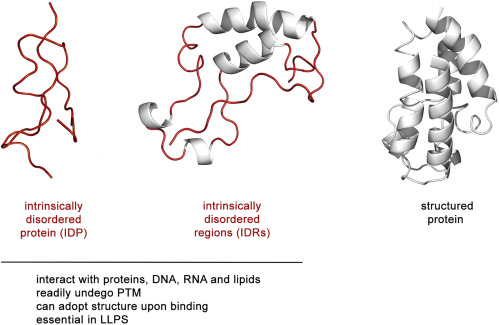
\includegraphics[scale=0.8]{res/proteins_overview/disordered.png}
	\centering
	\caption{Intrinsically Disordered Proteins, from \cite{intrinsic}}
	\label{fig:intrinsic}
\end{figure}
In disordered proteins the cost of folding is higher and so the protein has a lesser degree of freedom in folding.

It has complex surfaces which means high specificity with low versatility. For specificity we mean that when 2 proteins fit together, we need 2 highly specific protein structures to fit together, since their shape is so complex, an average protein can't be a proper fit.

Low versatility is the opposite: since the shape is quite complex, it doesn't fit together with most proteins, hence it's not versatile.

Due to their complex structures, disordered proteins are less prone to environmental stress: they can preserve their function in unstable conditions, such as high temperature.

In cell regulation around 25\% of proteins are disordered, those are involved in highly dynamic and complex processes that require proteins with high specificity.

IDPs (Intrinsically Disordered Proteins) are really interesting to study, because they are implicated in several pathologies and due to their different functions they are involved in:
\begin{itemize}
	\item Regulatory functions;
	\item Central role in the assembly of macromolecular machines, such as ribosomes;
	\item Transport of molecules through nuclear pore;
	\item Binding: IDPs can participate in one-to-many and many-to-many interactions, where one IDP region binds to multiple molecules, potentially gaining very different structures in the bound state.
\end{itemize}
 They are also implicated in several pathological conditions, like cancer, cardiovascular diseases, and neurodegenerative diseases. 

Some of the first classes of IDPs were notable due to their pathological roles in neurodegenerative diseases.

\vspace{20em}

\pagebreak

\section{Computational Biology: Computer Science Applied to Biology}
The growing amount of data in the field of Molecular Biology brought the scientists to exploit Computer Science. Computers can process data way faster than human beings, and especially in this field, where we have so much information on DNA, genes and proteins, it's really useful to compute and process these pieces of informations faster and possibly with less errors.

This new field takes the name of Bioinformatics, the union of Biology, Computer Science and Statistics. Statistics is needed because most of the information isn't 100\% reliable, hence statistics methods are used.
The main fields of bioinformatics are:
\begin{itemize}
    \item \textbf{Structural data analysis}: its purpose is to predict the three-dimensional structures of proteins, nucleic acids and other biological molecules. Understanding the structure of these molecules can provide insights into their functions and interactions;
    \item \textbf{Omics data analysis}: for example genomics, proteomics, metagenomics, epigenomics and so on. Omics data is a broad term that refers to large-scale datasets generated from various biological technologies. These large-scale datasets enable researchers to study different aspects of biological systems, often on a global or comprehensive scale. For example, in genomics analysis, we have large-scale datasets focused on genome data, so we can analyze DNA sequences and genes organization and functions.
\end{itemize}

In this thesis the focus will be on structural data analysis, since the software tool I talk about analyzes the three-dimensional structure to obtain information on the disorder or binding propensity.

\vspace{5em}
\pagebreak

\subsection{Structural Data}

\begin{figure}[h!]
    \centering
    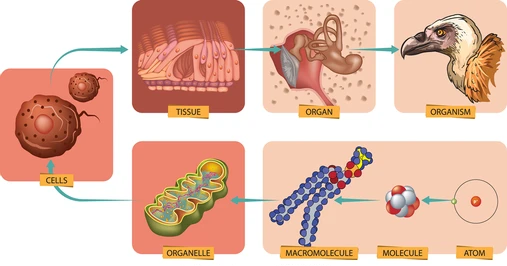
\includegraphics{res/proteins_overview/atom_bird.png}
    \caption{Atom to macromolecules to organism, from \cite{atombird}}
    \label{fig:atom-bird}
\end{figure}

In figure \ref{fig:atom-bird} we can see the various steps from molecules to macromolecules to bigger complexes up to the final organism.

We can use structural data for:
\begin{itemize}
    \item Structure prediction;
    \item Predicting protein interactions: protein folding, binding, protein assemblies;
    \item Structure comparison: by comparing the moolecules' structure we can determine to which species it belongs to and where in the evolutionary scale it stands;
    \item Exploring mechanisms of interaction with ligands: metabolites, drug compounds, DNA and others.
\end{itemize}

From molecular data we get information on coordinates and then we want to obtain some kind of knowledge, for example:
\begin{itemize}
    \item Mutation X disrupts the function of enzyme Y which causes disease Z.
\end{itemize}

\vspace{1em}

\noindent "Coordinates by themselves just specify shape and are not necessarily of intrinsic biological value, unless they can be related to other information"

\noindent \small{\textit{Integrative database analysis in structural genomics, Mark Gerstein, Nature Structural Biology}}

\pagebreak

\normalsize{There are many databases that store information on structural data for many proteins or other macromolecules, some of them also contains sequence data or metabolic pathways data. Sequence data are just data on DNA so the sequences, while metabolic pathways are related to which pathway a given gene activate.}

Down below we can see a picture of most databases for bioinformatics data.

The first database for structural data was PDB (Protein Data Bank), with the purpose of building an archive on protein structural data. A lot of the newer databases for structural data are derived from PDB.

Lastly, we can see a figure representing the most used biological technologies for obtaining structural data.

\begin{figure}[h!]
    \centering
    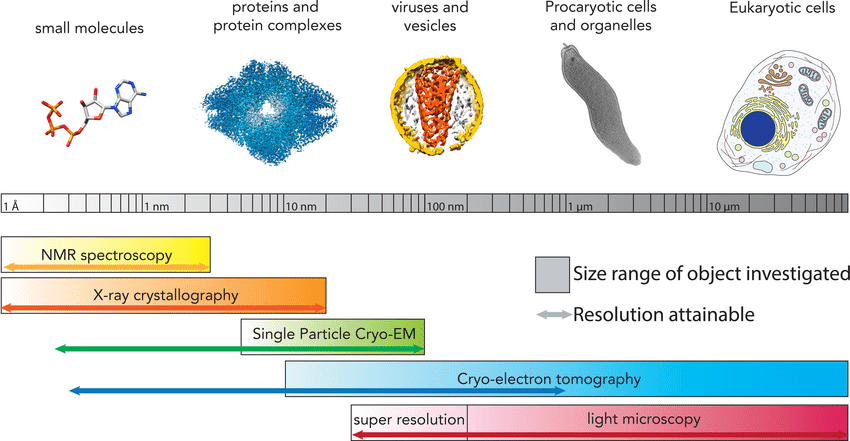
\includegraphics[scale=0.6]{res/proteins_overview/methods_structural.png}
    \caption{Biological technologies for obtaining structural data, from \cite{biotechs}}
\end{figure}

In our case, for protein chains and residues, the most interesting biological technologies are the first two from left:
\begin{itemize}
    \item X-ray crystallography;
    \item NMR spectroscopy.
\end{itemize}

To close up this chapter I will talk about one of the most important libraries in bioinformatics: BioPython.

\pagebreak

\subsection{BioPython}
Regarding Computer Science the main languages used for bioinformatics are:
\begin{itemize}
    \item R;
    \item Matlab;
    \item Python.
\end{itemize}
For python there is the library BioPython, which is a library containing classes, functions and modules for the various necessities in bioinformatics.

\begin{figure}[h!]
    \centering
    
\includegraphics{res/proteins_overview/biopython.png}
    \caption{BioPython logo}
\end{figure}

There are a lot of subpackages under the package Bio of BioPython, in our case we are just interested in 3 of them:
\begin{itemize}
    \item \textbf{Bio.PDB}: contains classes that deal with macromolecular crystal structures. In particular it includes PDB and mmCIF parsers, the DSSP wrapper\footnote{A wrapper is a class or procedure that translates a library's existing interface into a compatible interface, it "wraps" the underlying library. It's often used to enable cross-language, in this case the wrapper enables the c++ library "DSSP" to be used in Python.}, the SASA module and the Structure class;
    \item \textbf{Bio.Data}: collection of useful biological data, for example in our case we use it for the normalization factors for RSA;
    \item \textbf{Bio.SeqUtils}: contains mhelper functions to deal with sequences.
\end{itemize}

In particular from Bio.PDB we use the classes:
\begin{itemize}
    \item \textit{PDBParser}: as the name suggests, it's a class which reads a .pdb file and saves it into a variable of the type Structure class;
    \item \textit{MMCIFParser}: similar to PDBParser, but for .mmCIF files;
    \item \textit{DSSP}: the python wrapper for the software tool DSSP;
    \item \textit{SASA}: a class for calculating solvent accessibility;
    \item \textit{Polypeptide}: a class with helper functions to deal with protein chains, in particular we use the function \textbf{is\_aa()} to see if a string is an identifier for an amino acid.
\end{itemize}

On the other hand the Bio.Data subpackage has been used just for the normalization factors for SASA, the dictionary \textit{residue\_sasa\_scales}. 

And Bio.SeqUtils has been used for the helper function \textit{Seq1}, which converts a sequence of amino acids with three-letters code into a sequence of amino acids with one-letter code.

For more information on BioPython and its subpackages and submodules, here is the link to the  \underline{\href{https://biopython.org/docs/dev/api/index.html}{documentation}}.

\subsection{DSSP}

In BioPython we have an important procedure: the DSSP wrapper. DSSP (Define Secondary Structure Prediction) is a computer database used in structural bioinformatics to analyze a protein chain, in particular the secondary structure and other statistics that can be derived from it.

It uses hydrogen bond patterns and other geometric features of the protein to analyze it.